% =============================================================================
% Part I, Chapter 3: The Theoretical Foundations
% =============================================================================
\chapter{The Theoretical Foundations}\label{ch:theory}

To follow CausalFade's experimental journey from its early confounded backdoor tables to its final target-population transport benchmark, a reader needs tools from four disciplines that rarely share a single textbook: \emph{structural causal inference}, \emph{cognitive psychometrics}, \emph{low-bit weight quantization}, and \emph{clustered experimental statistics}. In this chapter, we build each concept from the ground up using a six-part layered exposition: (1) intuitive explanation, (2) formal scientific definition, (3) mathematical formulation, (4) concrete application inside CausalFade, (5) actual empirical evidence from the cohorts, and (6) scientific limitations.

\begin{figure}[htbp]
  \centering
  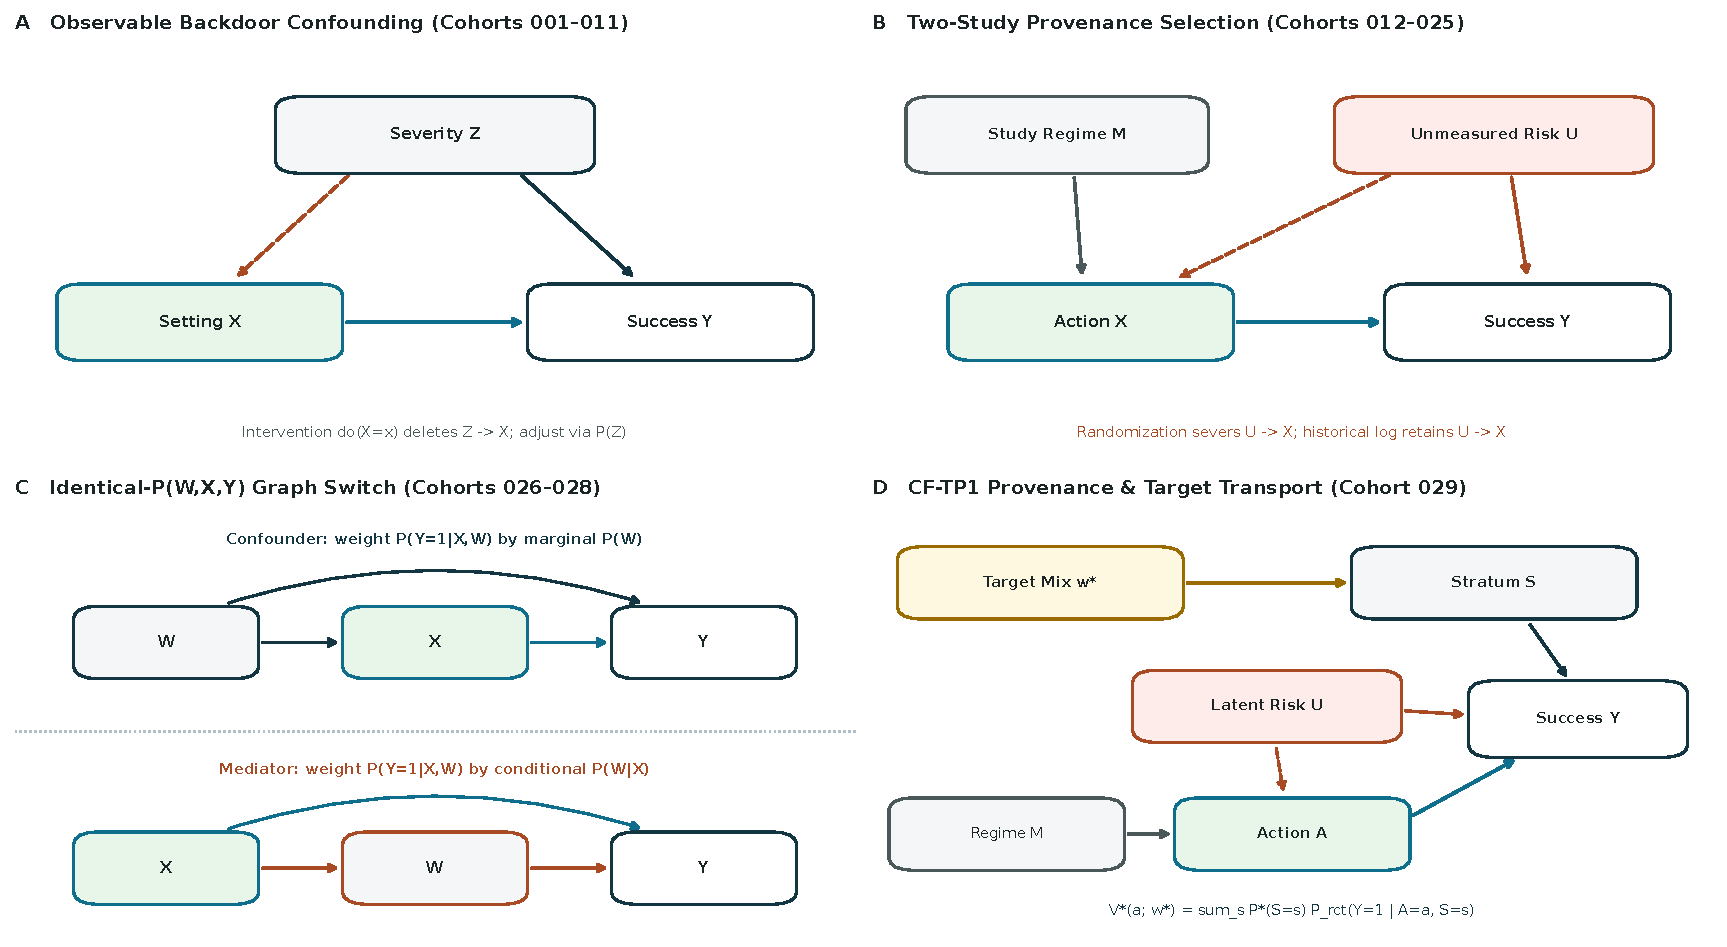
\includegraphics[width=\textwidth]{figures/fig08_structural_causal_diagrams.pdf}
  \caption{The four structural causal graph architectures investigated across Project CausalFade: (A) Observable backdoor confounding $Z\to X,Y$ (Cohorts~001--011); (B) Two-study randomized vs.\ unmeasured-confounder historical evidence (Cohorts~012--025); (C) Observationally equivalent confounder vs.\ mediator structures on identical $P(W,X,Y)$ tables (Cohorts~026--028); and (D) Selection diagram for target-population causal transport under stratum-mix shift (\texttt{CF-TP1}, Cohort~029).}
  \label{fig:scms}
\end{figure}

% =============================================================================
\section{Structural Causal Models, DAGs, and Conditional Independence}

\subsection{Intuitive Explanation}
Ordinary probability distributions describe \emph{which variables move together}, not \emph{which variable pushes which}. If severe machine wear ($Z=1$) prompts human operators to turn on an emergency cooling mode ($X=1$) and also causes frequent breakdowns ($Y=0$), then $X=1$ and $Y=0$ co-occur in historical logs even when cooling actually \emph{helps} every machine. A \textbf{Structural Causal Model (SCM)} writes down the directional data-generating mechanisms of the world as asymmetric assignments ($Y \leftarrow f_Y(X,Z,U_Y)$, read as ``nature computes $Y$ from $X$, $Z$, and exogenous noise $U_Y$''), while a \textbf{Directed Acyclic Graph (DAG)} draws those direct functional dependencies as arrows without feedback loops.

\subsection{Formal Scientific Definition and Mathematical Formulation}
\begin{definition}[Structural Causal Model and Induced Observational Law \citep{pearl2009causality}]
A Markovian Structural Causal Model is a tuple $\mathcal{M} = \langle \mathcal{U}, \mathcal{V}, \mathcal{F}, \Prob(\mathcal{U}) \rangle$, where $\mathcal{V} = \{V_1,\dots,V_m\}$ are endogenous variables, $\mathcal{U} = \{U_1,\dots,U_m\}$ are mutually independent exogenous background variables governed by product measure $\Prob(\mathcal{U}) = \prod_{j=1}^m \Prob(U_j)$, and $\mathcal{F} = \{f_1,\dots,f_m\}$ is a collection of structural equations
\begin{equation}
  V_j \coloneqq f_j(\mathrm{pa}_j, U_j), \qquad j = 1,\dots,m,
\end{equation}
whose parent sets $\mathrm{pa}_j \subseteq \mathcal{V}\setminus\{V_j\}$ form a Directed Acyclic Graph $\mathcal{G} = (\mathcal{V}, \mathcal{E})$ with directed edges $W \to V_j$ for each $W \in \mathrm{pa}_j$. Every Markovian SCM induces a unique joint observational distribution factoring along $\mathcal{G}$:
\begin{equation}
  \Prob_{\mathcal{M}}(v_1,\dots,v_m) = \prod_{j=1}^m \Prob(v_j \mid \mathrm{pa}_j).
  \label{eq:markov_factorization}
\end{equation}
\end{definition}

Conditional independence $A \Ind B \mid C$ means $\Prob(A,B\mid C) = \Prob(A\mid C)\Prob(B\mid C)$. In a DAG $\mathcal{G}$, Pearl's graphical criterion of \textbf{$d$-separation} characterizes every structural conditional independence implied by~\eqref{eq:markov_factorization}: a set of nodes $C$ blocks a path between $A$ and $B$ iff the path contains either a chain $i \to m \to j$ or fork $i \leftarrow m \to j$ with $m \in C$, or a collider $i \to c \leftarrow j$ such that neither $c$ nor any descendant of $c$ lies in $C$.

\subsection{Application, Evidence, and Limitations in CausalFade}
Figure~\ref{fig:scms} displays the four specific DAG architectures instantiated across CausalFade's 29 cohorts. In Cohorts~001--011 (Figure~\ref{fig:scms}A), $\mathcal{V} = \{Z, X, Y\}$ with fork $Z \leftarrow$ splitting into $Z \to X$ and $Z \to Y$ alongside causal edge $X \to Y$; conditioning on $Z$ blocks the noncausal backdoor path $X \leftarrow Z \to Y$. Conversely, in Cohorts~026--028 (Figure~\ref{fig:scms}C), when $W$ is a \emph{mediator} on the directed path $X \to W \to Y$, conditioning on $W$ blocks part of the desired causal effect rather than removing confounding! Empirically, Cohort~001 showed \texttt{Qwen2.5-3B F16} outputting \texttt{"adjustment\_set": ["X"]} ($0/64$ valid adjustment sets), conditioning on the treatment variable itself rather than the confounder $Z$, while Cohort~028 showed \texttt{Qwen2.5-7B F16} and \texttt{Llama-3.1-8B F16} choosing between \texttt{marginal} and \texttt{conditional} weighting at near-chance rates ($68/128$ and $60/128$) despite explicit DAG descriptions in the prompt. \emph{Limitation:} DAGs encode qualitative conditional independence and causal ancestry; as Cohorts~026--028 proved via exact rational tables, two distinct DAGs ($W\to X,Y$ vs.\ $X\to W\to Y$) can generate the \emph{exact same} observational joint table $\Prob(W,X,Y)$, meaning observational numbers alone can never identify the graph without external structural or temporal knowledge.

% =============================================================================
\section{Observational vs.\ Interventional Distributions and Pearl's \texorpdfstring{$\doop$}{do}-Operator}

\subsection{Intuitive and Formal Explanation}
Observing $X=x$ (\emph{seeing}) updates our beliefs about upstream causes of $X$: seeing an operator activate emergency cooling tells us the machine was probably already overheating. Intervening $\doop(X=x)$ (\emph{doing}) surgically overrides the operator's decision mechanism, forcing $X \coloneqq x$ for every unit regardless of initial state. Graphically, $\doop(X=x)$ deletes all incoming arrows into $X$ while leaving every other structural equation untouched.

\subsection{Mathematical Formulation: Truncated Factorization, ATE, CATE, and Simpson's Reversal}
In SCM $\mathcal{M}$, replacing $X \coloneqq f_X(\mathrm{pa}_X, U_X)$ with constant assignment $X \coloneqq x$ defines the mutilated submodel $\mathcal{M}_x$, whose interventional distribution obeys the \textbf{truncated factorization}:
\begin{equation}
  \Prob(v_1,\dots,v_m \mid \doop(X=x)) = \mathbb{I}(v_X = x) \prod_{V_j \neq X} \Prob(v_j \mid \mathrm{pa}_j).
  \label{eq:truncated_factorization}
\end{equation}
When covariate set $Z$ satisfies the \textbf{backdoor criterion} relative to $(X,Y)$---meaning no node in $Z$ is a descendant of $X$ and $Z$ blocks every path between $X$ and $Y$ containing an arrow into $X$---summing~\eqref{eq:truncated_factorization} yields Pearl's \textbf{backdoor adjustment formula}:
\begin{equation}
  \Prob(Y=1 \mid \doop(X=x)) = \sum_{z} \Prob(Y=1 \mid X=x, Z=z)\,\Prob(Z=z),
  \label{eq:backdoor}
\end{equation}
provided positivity $\Prob(X=x\mid Z=z) > 0$ holds for all strata with $\Prob(Z=z)>0$. By contrast, the naive observational conditional probability weights those exact same stratum success rates by \emph{treatment-conditioned} covariate shares:
\begin{equation}
  \Prob(Y=1 \mid X=x) = \sum_{z} \Prob(Y=1 \mid X=x, Z=z)\,\Prob(Z=z \mid X=x).
  \label{eq:obs_expansion}
\end{equation}
Comparing~\eqref{eq:backdoor} and~\eqref{eq:obs_expansion} makes confounding bias algebraically transparent. Define the stratum-specific \textbf{Conditional Average Treatment Effect ($\CATE$)}, population \textbf{Average Treatment Effect ($\ATE$)}, and naive \textbf{Observational Risk Difference ($\RD_{\mathrm{obs}}$)} for binary $Y \in \{0,1\}$:
\begin{align}
  \tau(z) &= \Prob(Y=1\mid X=1,Z=z) - \Prob(Y=1\mid X=0,Z=z) \nonumber\\
          &= \E[Y \mid \doop(X=1), Z=z] - \E[Y \mid \doop(X=0), Z=z], \label{eq:cate}\\
  \ATE &= \E[Y \mid \doop(X=1)] - \E[Y \mid \doop(X=0)] = \sum_{z} \tau(z)\,\Prob(Z=z), \label{eq:ate}\\
  \RD_{\mathrm{obs}} &= \Prob(Y=1 \mid X=1) - \Prob(Y=1 \mid X=0). \label{eq:rd_obs}
\end{align}
When confounding shifts $\Prob(Z=1\mid X=1)$ far away from $\Prob(Z=1\mid X=0)$, $\ATE$ and $\RD_{\mathrm{obs}}$ can have \emph{strictly opposite signs} ($\ATE \cdot \RD_{\mathrm{obs}} < 0$), known as \textbf{Simpson's reversal}.

\begin{workedexample}[Actual CausalFade Cohort~001 World \texttt{world-0000}, Task \texttt{cb2060af78e213308f0e}]
In \texttt{results/design\_validation/public\_tasks.jsonl} (line~1, reused in Cohort~001), $\Prob(Z=0)=\Prob(Z=1)=0.5$, and the exact stratum quantities are:
\begin{itemize}
  \item $Z=0$ (mild): $\Prob(Y=1\mid X=0,Z=0)=0.833549$ (cell mass $0.442746$), $\Prob(Y=1\mid X=1,Z=0)=0.738055$ (cell mass $0.057254$). Thus $\tau(0) = 0.738055 - 0.833549 = -0.095494$ ($-9.55\pp$).
  \item $Z=1$ (severe): $\Prob(Y=1\mid X=0,Z=1)=0.261945$ (cell mass $0.057254$), $\Prob(Y=1\mid X=1,Z=1)=0.166451$ (cell mass $0.442746$). Thus $\tau(1) = 0.166451 - 0.261945 = -0.095494$ ($-9.55\pp$).
\end{itemize}
Here both strata suffer a $-9.55\pp$ causal harm from activating $X$, so $\ATE = 0.5(-0.095494) + 0.5(-0.095494) = -0.095494 < 0$ (optimal action: \texttt{activate=0}). Because operators disproportionately activate $X$ when $Z=1$ ($\Prob(Z=1\mid X=1) = 0.8855$), the naive observational difference is even more negative ($\RD_{\mathrm{obs}} = 0.2319 - 0.7681 = -0.5362$), forming an \emph{aligned-negative} cell ($T=0, S=0$). Flipping the operator selection propensity in line~3 (\texttt{28a407789b6fcdab736f}) so operators activate $X$ mainly when $Z=0$ reverses $\RD_{\mathrm{obs}}$ to $+0.3609 > 0$ while keeping $\ATE = -0.095494 < 0$ unchanged, creating a \emph{conflict} cell ($T=0, S=1$)!
\end{workedexample}

\begin{pedagogicalexample}[Constructed Teaching Example: Confounder vs.\ Mediator on Identical Numbers]
\emph{(Constructed with simple round numbers for classroom clarity; see Chapter~11 for actual Cohort~027 six-decimal tables.)} Suppose an observational dataset of $100$ machines has exact joint counts:
\begin{itemize}
  \item Among $X=0$ ($50$ units): $10$ have $W=0$ ($8$ succeed, $80\%$) and $40$ have $W=1$ ($16$ succeed, $40\%$). Overall $X=0$ success is $(8+16)/50 = 48\%$.
  \item Among $X=1$ ($50$ units): $40$ have $W=0$ ($28$ succeed, $70\%$) and $10$ have $W=1$ ($3$ succeed, $30\%$). Overall $X=1$ success is $(28+3)/50 = 62\%$.
\end{itemize}
Notice that overall marginal prevalence is $\Prob(W=0) = (10+40)/100 = 0.50$ and $\Prob(W=1) = 0.50$.
\begin{enumerate}
  \item \textbf{Case A ($W$ is a pre-treatment confounder, $W \to X, Y$):} Intervening on $X$ does \emph{not} change $W$, so we weight by marginal $\Prob(W)=(0.5, 0.5)$: $\Prob(Y=1\mid \doop(X=0)) = 0.5(80\%) + 0.5(40\%) = 60\%$, while $\Prob(Y=1\mid \doop(X=1)) = 0.5(70\%) + 0.5(30\%) = 50\%$. Activating $X$ \emph{lowers} success by $-10\pp$ (\textbf{choose $X=0$}).
  \item \textbf{Case B ($W$ is a post-treatment mediator, $X \to W \to Y$, no unmeasured confounding):} Activating $X$ \emph{causes} $W=0$ to rise from $20\%$ to $80\%$, so the total interventional effect uses $\Prob(W\mid X=x)$: $\Prob(Y=1\mid \doop(X=0)) = \Prob(Y=1\mid X=0) = 48\%$, while $\Prob(Y=1\mid \doop(X=1)) = \Prob(Y=1\mid X=1) = 62\%$. Activating $X$ \emph{raises} success by $+14\pp$ (\textbf{choose $X=1$}).
\end{enumerate}
Same table, opposite optimal interventions! This exact mathematical duality drove Cohorts~026--028.
\end{pedagogicalexample}

% =============================================================================
\section{Randomized Evidence, Target-Population Transport, and Pairwise Fidelity}

\subsection{Intuitive Explanation}
Why did CausalFade evolve from single-table backdoor adjustment (Cohorts~001--011) and two-study aggregate comparisons (Cohorts~012--025) to \textbf{target-population transportability} in Cohort~029 (\texttt{CF-TP1})? In two-study aggregate tasks, once a model picks the randomized study, all that remains is comparing two printed numbers (\texttt{off 54.11\%, on 45.89\%})---a trivial single-inequality check easily mimicked by magnitude heuristics. Real-world policy decisions are harder in a structurally fundamental way:
\begin{enumerate}
  \item We have \textbf{two studies}: a historical study corrupted by unmeasured operator selection risk $U$, and a randomized trial where random assignment severs $U \to A$.
  \item Treatment helps one pre-treatment subgroup (say, \texttt{Blue}) and hurts another (\texttt{Amber})---known as \emph{qualitative CATE heterogeneity}.
  \item The \textbf{target population} where we must deploy the policy has its own subgroup composition $(w^*, 1-w^*)$, which differs from historical enrollment!
\end{enumerate}

\subsection{Formal Definition and Mathematical Formulation}
Let $S \in \{0,1\}$ denote a pre-treatment baseline group (\texttt{Amber} $=0$, \texttt{Blue} $=1$), $U \in \{0,1\}$ an unmeasured risk factor, $M \in \{\mathrm{rct}, \mathrm{hist}\}$ the study regime, $A \in \{0,1\}$ the treatment action, and $Y \in \{0,1\}$ success (Figure~\ref{fig:scms}D).
\begin{itemize}
  \item Under the \textbf{randomized study} ($M=\mathrm{rct}$), $A \Ind U \mid S$, so observed group-specific rates identify true stratum potential-outcome expectations:
  \begin{equation}
    \mu_{\mathrm{rct}}(s, a) = \Prob(Y=1 \mid M=\mathrm{rct}, S=s, A=a) = \E[Y(a) \mid S=s].
  \end{equation}
  \item Under the \textbf{historical study} ($M=\mathrm{hist}$), operators choose $A$ partly based on unmeasured risk $U$ ($U \to A$ and $U \to Y$), so $\mu_{\mathrm{hist}}(s, a) = \Prob(Y=1 \mid M=\mathrm{hist}, S=s, A=a) \neq \E[Y(a) \mid S=s]$ even within stratum $S=s$!
  \item Under \textbf{stratum transportability} \citep{pearl2014external,westreich2017transportability}---conditional causal effects $\E[Y(a)\mid S=s]$ carry over unchanged to a target population $\Pi^*$ with known stratum share $w^* = \Prob^*(S=0) \in (0,1)$---the target interventional value of action $a$ and standardized causal effect $\tau^*(w^*)$ are:
  \begin{align}
    V^*(a; w^*) &= \Prob^*(Y=1 \mid \doop(A=a)) = w^*\,\mu_{\mathrm{rct}}(0,a) + (1-w^*)\,\mu_{\mathrm{rct}}(1,a), \label{eq:transport_val}\\
    \tau^*(w^*) &= V^*(1; w^*) - V^*(0; w^*) = w^*\,\delta_{\mathrm{rct}}(0) + (1-w^*)\,\delta_{\mathrm{rct}}(1), \label{eq:transport_ate}
  \end{align}
  where $\delta_{\mathrm{rct}}(s) = \mu_{\mathrm{rct}}(s,1) - \mu_{\mathrm{rct}}(s,0)$. Whenever $\delta_{\mathrm{rct}}(0)$ and $\delta_{\mathrm{rct}}(1)$ have opposite signs, $\tau^*(w^*)$ is an affine function of $w^*$ that crosses zero at the interior threshold
  \begin{equation}
    w_{\mathrm{crit}} = \frac{-\delta_{\mathrm{rct}}(1)}{\delta_{\mathrm{rct}}(0) - \delta_{\mathrm{rct}}(1)} \in (0,1).
    \label{eq:w_crit}
  \end{equation}
\end{itemize}

Consequently, evaluating the \emph{exact same two study tables} at two target population mixes $w_0 < w_{\mathrm{crit}} < w_1$ forces a causally competent decision-maker to \textbf{reverse} its optimal action $a^*(w) = \mathbb{I}(\tau^*(w) > 0)$! Conversely, if two target mixes lie on the same side of $w_{\mathrm{crit}}$ (or if both strata share the same sign in one of the balanced sign-matrix strata), the optimal decision must be \textbf{retained} (invariance). Figure~\ref{fig:transport_f096} illustrates this exact geometry on Cohort~029's archived Family~\texttt{096}.

\begin{figure}[htbp]
  \centering
  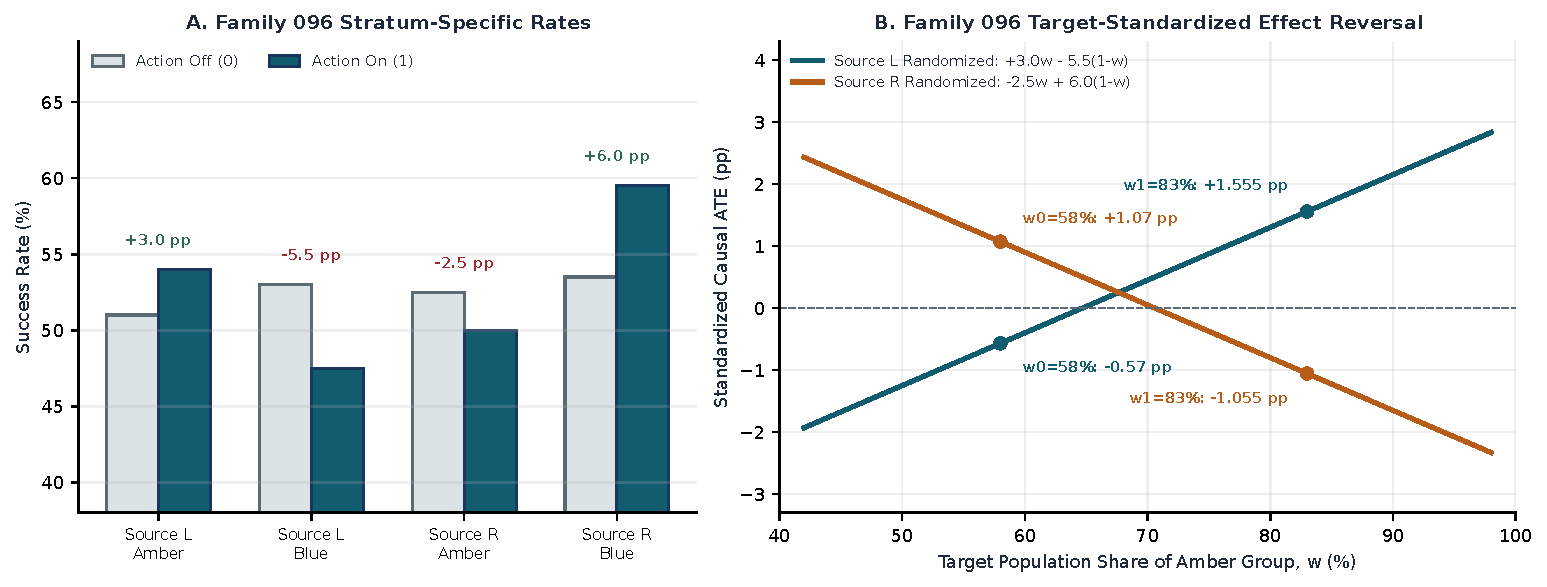
\includegraphics[width=\textwidth]{figures/fig10_target_population_transport.pdf}
  \caption{Target-population causal transport in archived \texttt{CF-TP1} Family~\texttt{096} (\texttt{experiments/cohort\_029/freeze/fixture/worlds.jsonl}): (A) Stratum-specific off/on percentages in Source~L and Source~R; (B) Standardized causal effect lines $\tau_k(w)$ reversing sign between Mix~0 ($w_0=58\%$) and Mix~1 ($w_1=83\%$).}
  \label{fig:transport_f096}
\end{figure}

\subsection{Decision Reversal, Retention, and Pairwise Fidelity}
Consider any pair of minimally contrasted tasks $(x_0, x_1)$ with gold binary actions $(g_0, g_1) \in \{0,1\}^2$ and model predictions $(\hat{a}_0, \hat{a}_1) \in \{0,1\}^2$. Let $I_m = \mathbb{I}(\hat{a}_m = g_m)$ be single-item correctness on member $m \in \{0,1\}$.
\begin{itemize}
  \item \textbf{Single-item accuracy} $\frac{1}{2}(I_0 + I_1)$ awards $50\%$ credit on every reversal pair ($g_0 \neq g_1$) to a degenerate constant policy ($\hat{a}_0 = \hat{a}_1 = 1$), because any constant answer matches whichever member happens to have gold label $1$!
  \item \textbf{Pairwise bundle fidelity} \citep{gardner2020contrast} scores $1$ iff \emph{both} members of the pair are answered correctly:
  \begin{equation}
    F_{\mathrm{pair}}(x_0, x_1) = I_0 \cdot I_1 = \mathbb{I}(\hat{a}_0 = g_0 \;\wedge\; \hat{a}_1 = g_1).
    \label{eq:pair_fidelity}
  \end{equation}
\end{itemize}
On a \textbf{switch pair} ($g_0 \neq g_1$), $F_{\mathrm{pair}} = 1$ requires both switching ($\hat{a}_0 \neq \hat{a}_1$) \emph{and} getting the direction right ($\hat{a}_0 = g_0$); any constant policy ($\hat{a}_0 = \hat{a}_1$) receives $F_{\mathrm{pair}} = 0$! Simultaneously, including an equal number of \textbf{invariant pairs} ($g_0 = g_1$) prevents an adversarial heuristic that blindly alternates answers across pairs from gaming switch pairs, because blind alternation scores $F_{\mathrm{pair}} = 0$ on invariant pairs (Figure~\ref{fig:reversal_retention}).

\begin{figure}[htbp]
  \centering
  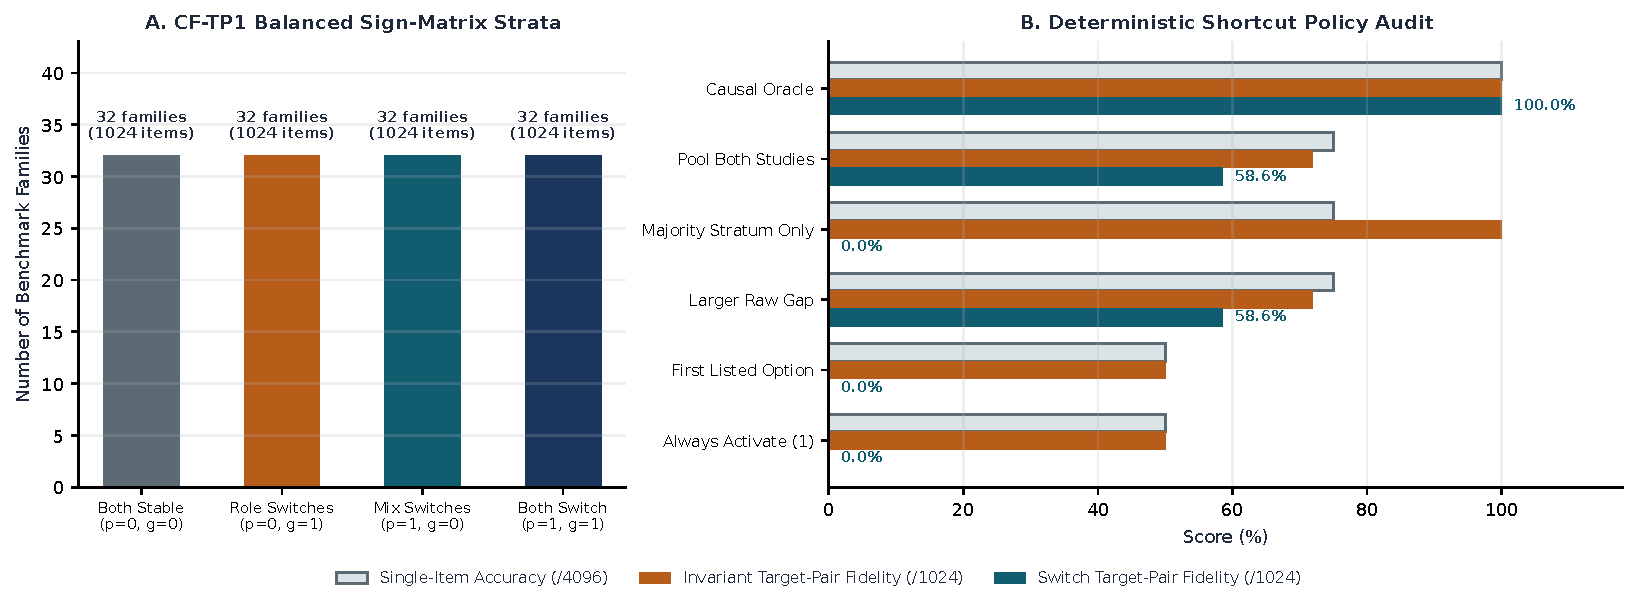
\includegraphics[width=\textwidth]{figures/fig11_decision_reversal_retention.pdf}
  \caption{Balanced sign-matrix design and shortcut policy audit in \texttt{CF-TP1}: (A) Four $32$-family sign-matrix strata $(p,g)\in\{0,1\}^2$ balancing reversal and invariance across target-mix and source-role axes; (B) Why single-item accuracy ($50\%$) and invariant pairs ($50\%$) fail to expose constant-activation or option-order policies, whereas switch-pair fidelity drives constant policies to $0\%$.}
  \label{fig:reversal_retention}
\end{figure}

% =============================================================================
\section{Psychometric Decompositions: C/A/B Trees and Signal Detection Theory}

\subsection{The C/A/B Multinomial Processing Tree---and Why It Failed}
Adapted from \citet{jacoby1991process} and \citet{gawronski2017cni} during \texttt{design\_validation} (\texttt{causalfade/cab\_tree.py}), the 3-parameter Causal/Associative/Bias ($C/A/B$) tree models the probability of choosing \texttt{activate=1} given causal cue $T \in \{0,1\}$ and associative cue $S \in \{0,1\}$ as:
\begin{equation}
  \Prob(\text{act}=1 \mid T, S) = p_{TS} = C \cdot T + (1 - C)\bigl[A \cdot S + (1 - A) B\bigr], \qquad C, A, B \in [0,1].
  \label{eq:cab_tree}
\end{equation}
Expanding~\eqref{eq:cab_tree} over $(T,S) \in \{0,1\}^2$ yields four linear equations in $(w_C, w_A, w_B) = (C, (1-C)A, (1-C)(1-A)B)$:
\begin{align}
  p_{11} &= C + (1-C)A + (1-C)(1-A)B, & p_{10} &= C + (1-C)(1-A)B, \nonumber\\
  p_{01} &= (1-C)A + (1-C)(1-A)B,     & p_{00} &= (1-C)(1-A)B. \label{eq:cab_cells}
\end{align}
Because four binomial cell probabilities $(p_{11}, p_{10}, p_{01}, p_{00})$ are fitted by three parameters,~\eqref{eq:cab_cells} imposes an exact \textbf{zero-interaction additivity constraint}:
\begin{equation}
  \mathcal{I}_{\mathrm{tree}} \coloneqq p_{11} - p_{10} - p_{01} + p_{00} = 0.
  \label{eq:cab_additivity}
\end{equation}
Two fatal limitations surfaced immediately in CausalFade (Figure~\ref{fig:cab_recovery}):
\begin{enumerate}
  \item \textbf{Observational equivalence to continuous cue integration (\texttt{design\_validation}):} Any symmetric additive logistic model $\Prob(\text{act}=1\mid T,S) = \sigma\bigl(\beta_T(2T-1) + \beta_S(2S-1)\bigr)$ with zero intercept satisfies $p_{00} + p_{11} = 1$ and $p_{10} + p_{01} = 1$, which algebraically implies $p_{11} - p_{10} - p_{01} + p_{00} = (1-p_{00}) - p_{10} - (1-p_{10}) + p_{00} = 0$! Hence a 4-cell table can \emph{never} distinguish sequential discrete gating ($C \to A \to B$) from simultaneous weighted evidence summation ($p_{\text{boot}} = 0.433$).
  \item \textbf{Empirical violation of additivity (Cohort~005):} On \texttt{Qwen2.5-3B F16}, observed cell probabilities yielded $\widehat{\mathcal{I}}_{\mathrm{tree}} = -0.4375$ ($-43.75\pp$, 95\% CI $[-68.75, -18.75]\pp$), decisively falsifying cross-cell parameter invariance.
\end{enumerate}

\begin{figure}[htbp]
  \centering
  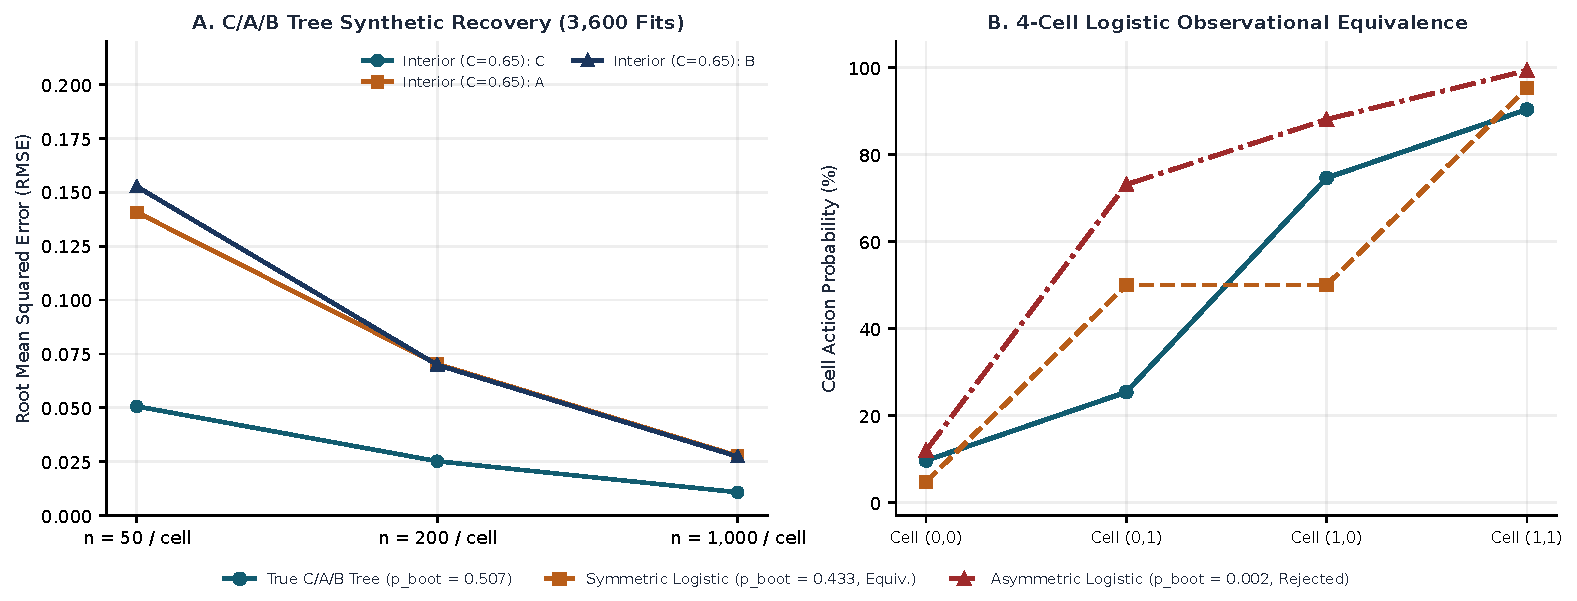
\includegraphics[width=\textwidth]{figures/fig18_synthetic_cab_recovery.pdf}
  \caption{Pre-LLM synthetic validation of the $C/A/B$ processing tree (\texttt{results/design\_validation/parameter\_recovery.json}, $3{,}600$ EM fits): (A) RMSE across cell sizes $n\in\{50,200,1000\}$ showing inflation of conditional parameter error when $C$ is high or $n$ is small; (B) Exact observational equivalence between the discrete $C/A/B$ tree and symmetric logistic cue integration ($p_{\text{boot}}=0.433$).}
  \label{fig:cab_recovery}
\end{figure}

\subsection{Signal Detection Theory (\texorpdfstring{$d'$}{d'} and Criterion \texorpdfstring{$c$}{c})}
To summarize binary sensitivity and directional response bias without assuming sequential latent branches, Cohort~024 adopted \textbf{Signal Detection Theory} \citep{jones2016cue}. Defining the hit rate $H = \Prob(\hat{a}=1 \mid g=1)$ and false-alarm rate $F = \Prob(\hat{a}=1 \mid g=0)$ (with log-linear / half-count boundary smoothing $(k+0.5)/(n+1)$ so $\Phi^{-1}(\cdot)$ remains finite when $k=0$ or $k=n$), sensitivity $d'$ and decision criterion $c$ are:
\begin{equation}
  d' = \Phi^{-1}(H) - \Phi^{-1}(F), \qquad c = -\frac{1}{2}\bigl[\Phi^{-1}(H) + \Phi^{-1}(F)\bigr],
  \label{eq:sdt}
\end{equation}
where $\Phi^{-1}$ is the standard normal probit function. Here $d'=0$ indicates zero discrimination between beneficial ($g=1$) and harmful ($g=0$) interventions, $c < 0$ indicates liberal \texttt{activate=1} bias, and $c > 0$ indicates conservative \texttt{decline} (\texttt{activate=0}) bias.

% =============================================================================
\section{Floating-Point Precision and GGUF Block-Affine Quantization}

\subsection{Intuitive and Formal Explanation}
In unquantized half-precision (\texttt{F16}, IEEE~754 \texttt{binary16}), each neural network weight uses $16$ bits ($1$ sign bit, $5$ exponent bits, $10$ mantissa bits), representing values across $\sim 10^{-5}$ to $65{,}504$ with roughly $3.3$ significant decimal digits. \textbf{Post-Training Quantization (PTQ)} in the \texttt{llama.cpp} \texttt{GGUF} ecosystem partitions weight rows into small contiguous blocks (e.g., $32$ weights in \texttt{Q8\_0}, or $256$-weight ``super-blocks'' subdivided into $16$--$32$-weight sub-blocks in K-quants \texttt{Q6\_K}, \texttt{Q5\_K\_M}, \texttt{Q4\_K\_M}, \texttt{Q3\_K\_M}, \texttt{Q2\_K}) and stores low-bit integers alongside shared floating-point block scales and offsets.

\subsection{Mathematical Formulation and Bits-Per-Weight (\texorpdfstring{$\BPW$}{BPW})}
For a block $\mathbf{w} \in \mathbb{R}^B$ under symmetric $b$-bit quantization (such as \texttt{Q8\_0}, $B=32$, $b=8$), quantization and dequantization compute:
\begin{equation}
  s = \frac{\max_i |w_i|}{2^{b-1}-1}, \qquad q_i = \operatorname{round}\!\left(\frac{w_i}{s}\right) \in \{-127,\dots,127\}, \qquad \widehat{w}_i = s \cdot q_i.
\end{equation}
In asymmetric hierarchical K-quants (e.g., \texttt{Q4\_K\_M}, \texttt{Q2\_K}), a 256-weight super-block stores FP16 super-scales $(d, d_{\min})$, quantized 6-bit or 4-bit sub-block scales $(s_m, k_m)$, and $b$-bit integer weights $q_{m,j} \in \{0,\dots,2^b-1\}$, reconstructing
\begin{equation}
  \widehat{w}_{m,j} = (d \cdot s_m)\, q_{m,j} - (d_{\min} \cdot k_m), \qquad \text{with reconstruction error } \varepsilon_{m,j} = \widehat{w}_{m,j} - w_{m,j}.
  \label{eq:kquant}
\end{equation}
Because scale metadata and mixed-precision attention/output tensors (\texttt{\_M} suffix promotes sensitive tensors such as \texttt{attn\_v} or \texttt{ffn\_down} to higher bit-widths) add overhead beyond $b$ bits, effective compression is measured in \textbf{bits per weight ($\BPW$)}:
\begin{equation}
  \BPW = \frac{8 \times \text{TensorBytes}_{\mathrm{quantized}}}{N_{\mathrm{parameters}}}.
\end{equation}
Across CausalFade's inventory (Chapter~4), \texttt{F16} sits at $16.00\;\BPW$, \texttt{Q8\_0} at $\approx 8.50\;\BPW$, \texttt{Q6\_K} at $\approx 6.56\;\BPW$, \texttt{Q5\_K\_M} at $\approx 5.69\;\BPW$, \texttt{Q4\_K\_M} at $\approx 4.85\;\BPW$, \texttt{Q3\_K\_M} at $\approx 3.91\;\BPW$, and \texttt{Q2\_K} at $\approx 2.96\;\BPW$.

% =============================================================================
\section{Construct Validity, Shortcuts, Matched Controls, and Clustered Inference}

\subsection{Benchmark Shortcuts and Matched Experimental Controls}
A benchmark possesses \textbf{construct validity} iff high scores can be achieved \emph{only} by exercising the target cognitive or mathematical capability, and low scores reflect genuine deficits in that capability rather than extraneous formatting or arithmetic bottlenecks. Let $\mathcal{H}_{\mathrm{shortcut}}$ denote a class of deterministic surface policies that inspect printed numbers, token positions, or study order \emph{without} using causal identification rules. If there exists $h \in \mathcal{H}_{\mathrm{shortcut}}$ with high benchmark score, any LLM matching $h$ will appear ``causally competent'' for noncausal reasons \citep{mccoy2019right}. Conversely, if an LLM fails a causal task solely because it cannot multiply two percentages and add them, attributing that failure to ``lack of causal understanding'' commits the inverse construct-validity error. CausalFade resolved both sides of this trap by combining:
\begin{enumerate}
  \item \textbf{Pre-execution shortcut audits:} Proving over $162$ deterministic noncausal policies in Cohort~029 (\texttt{policy\_audit.json}) that no rule ignoring source provenance or target composition exceeds structural chance ceilings on pairwise fidelity; and
  \item \textbf{Matched noncausal controls:} Pairing every causal task with an isomorphic noncausal scorecard task over the \emph{exact same numbers, weights, options, and JSON output schema}, isolating causal identification overhead via the paired within-family difference $D_i = Y_{i,\mathrm{causal}} - Y_{i,\mathrm{control}}$.
\end{enumerate}

\subsection{Clustered Variance and Dual Parametric/Bounded Confidence Intervals}
Because each synthetic world family $i \in \{1,\dots,N\}$ generates multiple correlated prompt items (e.g., $32$ prompts and $8$ transfer target pairs per family in Cohort~029), treating individual prompts as independent Bernoulli trials ($n=4{,}096$) severely underestimates standard errors (pseudo-replication). The statistically valid unit of randomization and independence is the \textbf{world family cluster} $i$.

In Cohort~029's stratified design of $H=8$ equal strata of $m_h = 16$ independent families ($N = \sum_{h=1}^8 m_h = 128$), let $D_{hi} \in [-1, 1]$ denote the family-level causal-minus-arithmetic difference in transfer target-pair fidelity for family $i$ in stratum $h$, with stratum sample mean $\bar{D}_h = \frac{1}{m_h}\sum_{i=1}^{m_h} D_{hi}$ and stratum sample variance $s_h^2 = \frac{1}{m_h-1}\sum_{i=1}^{m_h}(D_{hi}-\bar{D}_h)^2$. The stratified estimator, standard error, and Welch--Satterthwaite degrees of freedom \citep{welch1947generalization} are:
\begin{equation}
  \widehat{\Delta} = \frac{1}{H}\sum_{h=1}^H \bar{D}_h, \qquad
  \widehat{\mathrm{SE}}(\widehat{\Delta}) = \sqrt{\sum_{h=1}^H \frac{s_h^2}{H^2 m_h}}, \qquad
  \hat{\nu} = \frac{\left(\sum_{h=1}^H \frac{s_h^2}{H^2 m_h}\right)^2}{\sum_{h=1}^H \frac{(s_h^2 / (H^2 m_h))^2}{m_h - 1}},
  \label{eq:strat_welch}
\end{equation}
yielding the $95\%$ Welch $t$ interval $\widehat{\Delta} \pm t_{0.975, \hat{\nu}}\,\widehat{\mathrm{SE}}(\widehat{\Delta})$. Simultaneously, because $D_{hi} \in [-1, 1]$ has bounded range $b - a = 2$, Hoeffding's inequality \citep{hoeffding1963probability} guarantees finite-sample $(1-\alpha)$ coverage via the distribution-free radius
\begin{equation}
  r_{\mathrm{bounded}}(\alpha) = (b - a)\sqrt{\frac{\ln(2/\alpha)}{2 N}} = 2\sqrt{\frac{\ln(2/0.05)}{2 \times 128}} = 2\sqrt{\frac{\ln 40}{256}} \approx 0.240081 \;\;(24.01\pp),
  \label{eq:hoeffding_radius}
\end{equation}
producing Cohort~029's exact archived bounded interval $\widehat{\Delta} \pm 0.240081 = [-27.52\pp, +20.49\pp]$ (\texttt{primary.json}). Notice how equation~\eqref{eq:hoeffding_radius} reproduces the exact archived radius $-0.03515625 - (-0.27523695) = 0.24008070$ to eight decimal places!
